% Shared preamble for the English summaries in this repository.
\documentclass[11pt,a4paper]{article}
\usepackage[margin=2.2cm]{geometry}
\usepackage[T1]{fontenc}
\usepackage[utf8]{inputenc}
\usepackage{lmodern}
\usepackage{amsmath,amssymb}
\usepackage{graphicx}
\usepackage{booktabs}
\usepackage{enumitem}
\usepackage[hidelinks]{hyperref}
\setlist{itemsep=2pt,topsep=4pt}
\setlength{\parindent}{0pt}
\setlength{\parskip}{5pt}
\graphicspath{{figures/}}
\newcommand{\summaryheader}[3]{%
  \begin{center}
    {\Large\bfseries #2}\\[3pt]
    {\large #1}\\[3pt]
    {\small Arshia Goshtasbi \textbullet{} MSc Electrical Engineering (Control), Iran University of Science and Technology \textbullet{} #3}
  \end{center}
  \vspace{2pt}\hrule\vspace{8pt}\par}

\begin{document}
\summaryheader{Reinforcement Learning, HW4--HW5 and Comprehensive Exercise Q1}{Tabular Reinforcement Learning on Gymnasium Tasks}{Autumn 1403 (2024)}

\section*{1. FrozenLake: six solution methods}
The deterministic $4\times4$ FrozenLake has 16 states and 4 actions; reaching the goal pays $+1$ and falling in a hole ends the episode. With $\gamma=0.95$ I solved it with two model-based and four model-free methods.

\begin{itemize}
  \item \textbf{Policy iteration.} Exact evaluation $V^{\pi}=(I-\gamma P_\pi)^{-1}r_\pi$, then greedy improvement $\pi(s)\leftarrow\arg\max_a \sum_{s'}p(s'|s,a)\,[r+\gamma V^\pi(s')]$. Converged in 7 iterations.
  \item \textbf{Value iteration.} $V_{k+1}(s)=\max_a\sum_{s'}p(s'|s,a)\,[r+\gamma V_k(s')]$, 7 sweeps to $10^{-10}$.
  \item \textbf{On-policy first-visit Monte Carlo} with an $\varepsilon$-soft policy, $\varepsilon$ decaying from 0.5 to 0.05 over 20{,}000 episodes.
  \item \textbf{Off-policy Monte Carlo} with weighted importance sampling: greedy target policy, $\varepsilon$-greedy behaviour ($\varepsilon=0.5$), $C(s,a)\mathrel{+}=W$, $Q\mathrel{+}=\tfrac{W}{C}(G-Q)$, $W\leftarrow W/b(a|s)$, stopping at the first non-greedy action.
  \item \textbf{SARSA} and \textbf{Q-learning} with $\alpha=0.5$ and $\varepsilon$ decaying linearly to 0.01.
\end{itemize}

All six greedy policies reach the goal in 100\% of rollouts. Policy and value iteration give the optimal action in all 11 non-terminal states; the model-free methods give it in 10--11, missing only states that the learned path rarely visits.

\begin{center}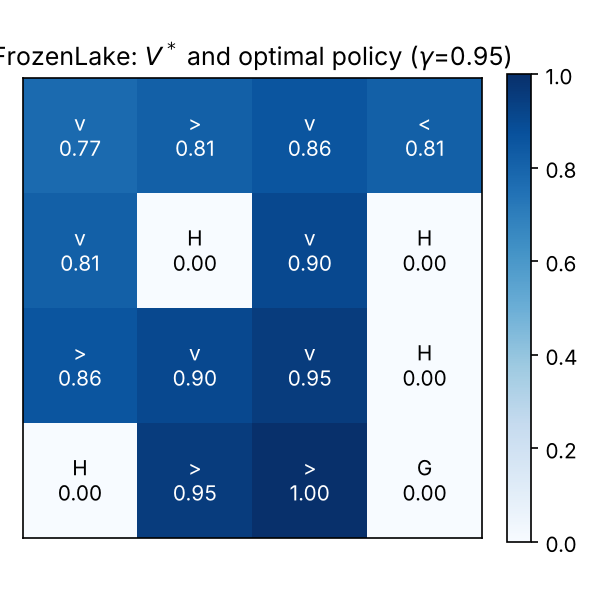
\includegraphics[width=0.38\textwidth]{frozenlake_value.png}\end{center}

\section*{2. MountainCar: Q-learning on a grid}
The continuous state (position, velocity) is binned on a $20\times20$ grid and Q-learning runs for 10{,}000 episodes with $\alpha=0.1$, $\gamma=0.99$ and $\varepsilon$ decaying from 0.5 to 0.01. The greedy policy reaches the flag from all 100 test starts, in a median of 137 steps.

\begin{center}
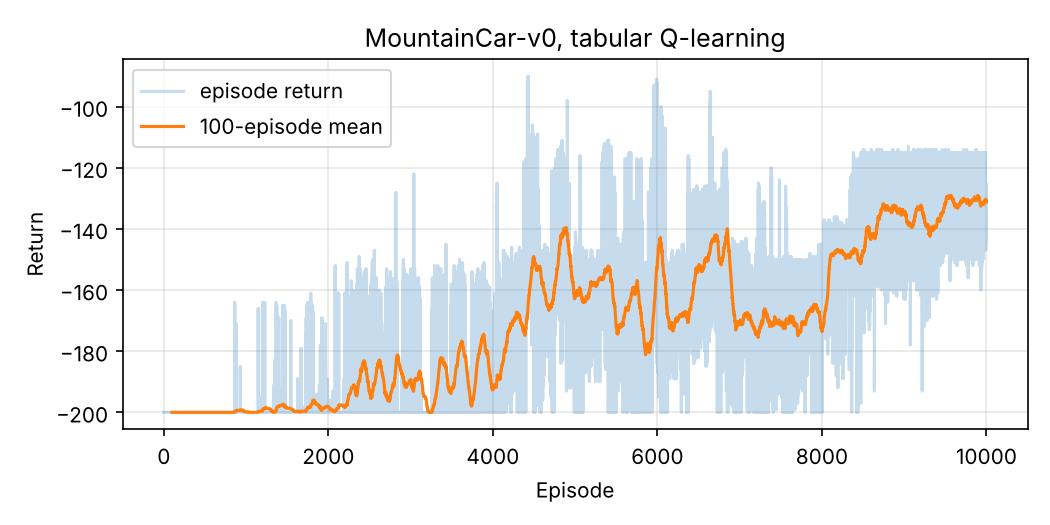
\includegraphics[width=0.56\textwidth]{mountain_car_learning_curve.png}\hfill
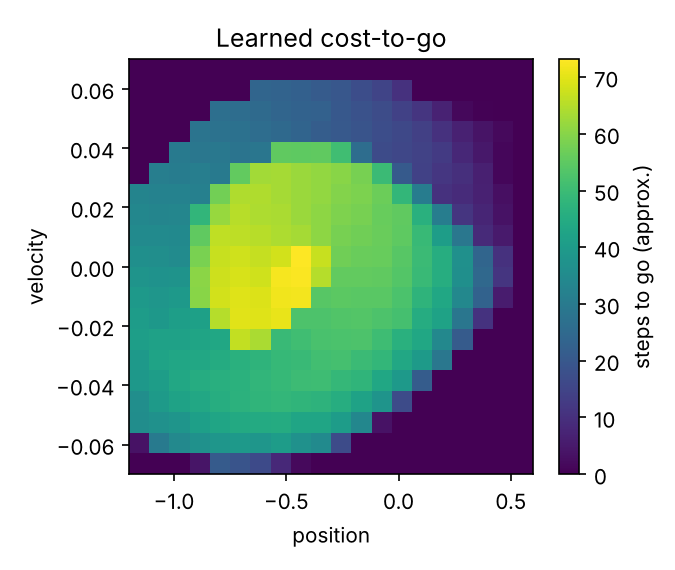
\includegraphics[width=0.38\textwidth]{mountain_car_value.png}
\end{center}

\section*{3. CartPole: Monte Carlo vs.\ Q-learning vs.\ SARSA}
All three methods share one grid ($3\times3\times12\times12$ cells over cart position, cart velocity, pole angle and angular velocity), $\gamma=0.99$, the same $\varepsilon$ schedule and 6{,}000 episodes, and each ran with three seeds. The greedy policies balanced the pole for these mean numbers of steps over 50 test episodes (500 is the limit):

\begin{center}
\begin{tabular}{lccc}\toprule
 & Seed 0 & Seed 1 & Seed 2\\\midrule
Every-visit Monte Carlo & 459.5 & 478.4 & 430.6\\
Q-learning & 500.0 & 500.0 & 186.2\\
SARSA & 500.0 & 257.8 & 296.0\\\bottomrule
\end{tabular}
\end{center}

The TD methods can reach the limit but depend strongly on the seed with a constant step size on a coarse grid. Monte Carlo, which averages complete returns, was the most consistent here.

\begin{center}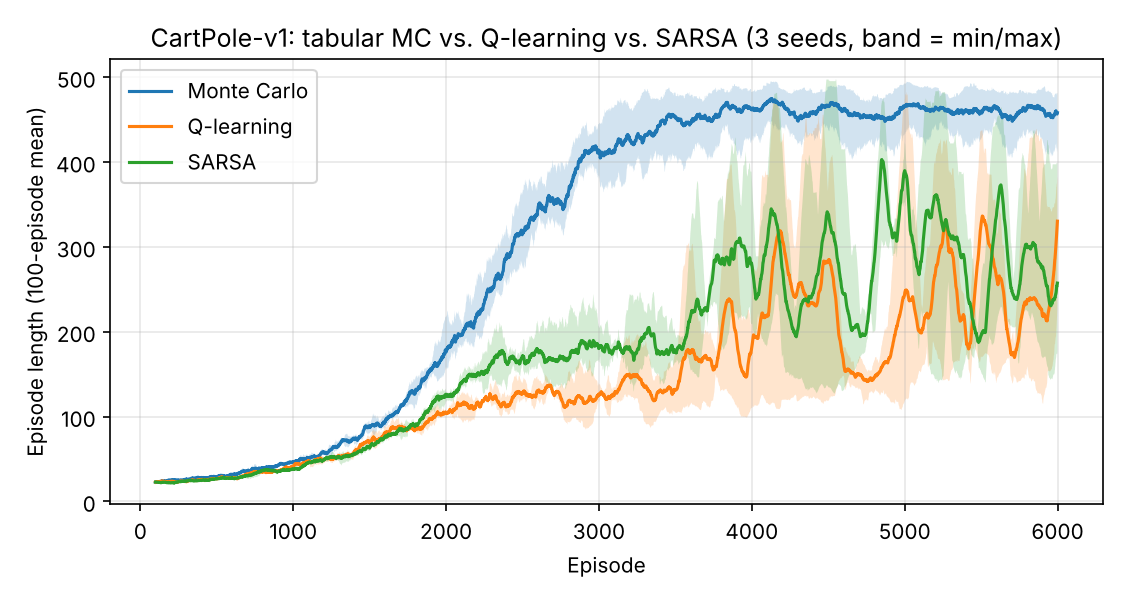
\includegraphics[width=0.8\textwidth]{cartpole_learning_curves.png}\end{center}
\end{document}
